\section{Experimental Setup}

\subsection{Datasets: Synthetic Benchmarks and Clinical Signals}
To systematically evaluate estimation performance across varying statistical complexities, we evaluate three experimental benchmarks.

\subsubsection{Linear Vector Autoregression (VAR) with Noise Corruption}
To benchmark asymptotic convergence against analytically tractable ground truth under measurement noise, we synthesize a bivariate vector autoregressive model:
\begin{align}
    x_t &= a_{11} x_{t-1} + a_{12} y_{t-1} + \epsilon_{x,t} + \xi_{x,t} \\
    y_t &= a_{21} x_{t-1} + a_{22} y_{t-1} + \epsilon_{y,t} + \xi_{y,t}
\end{align}
where $\epsilon_x, \epsilon_y \sim \mathcal{N}(0, \sigma_\epsilon^2)$ represent internal process innovations, while $\xi_x, \xi_y \sim \mathcal{N}(0, \sigma_\xi^2)$ introduce Additive White Gaussian Noise (AWGN). We configure unidirectional coupling ($a_{21} = 0.5, a_{12} = 0.0$), computing analytical ground truth via the exact stationary covariance matrix. We benchmark across Signal-to-Noise Ratios (SNR) $\in \{\infty \text{ (Clean)}, 20, 15, 10, 5, 0\text{ dB}\}$ across window sizes $N \in \{20, 50, 100\}$ (30 independent realization windows per condition).

\subsubsection{Non-linear Periodic Coupling}
To replicate the non-linear rhythmic oscillations characteristic of physiological processes, we generate coupled non-linear oscillators:
\begin{align}
    x_t &= \sin(\omega_x t) + \epsilon_{x,t} \\
    y_t &= \sin(\omega_y t) + C \cdot f(x_{t-\tau}) + \epsilon_{y,t}
\end{align}
where $C$ denotes coupling strength, $\tau = 1$ is the interaction delay, and $f(\cdot) = \tanh(\cdot)$ introduces strict non-linearity. This dataset serves as our primary benchmark for evaluating variance reduction in the small-sample regime ($N \in [10, 200]$).

\subsubsection{Complete 40-Subject PhysioNet Fantasia Database}
To validate real-world clinical efficacy, we evaluate the complete 40-subject cohort of the PhysioNet Fantasia database \cite{iyengar1996age, goldberger2000physiobank}. The cohort consists of:
\begin{itemize}
    \item \textbf{Young Cohort:} 20 subjects, ages $25.95 \pm 4.31$ years (range 21--34), balanced sex ratio (10 M / 10 F).
    \item \textbf{Old Cohort:} 20 subjects, ages $74.55 \pm 4.45$ years (range 68--85), balanced sex ratio (10 M / 10 F).
\end{itemize}
Simultaneous electrocardiogram (ECG) and continuous respiration signals were recorded during 2 hours of quiet supine resting. Signals are bandpass-filtered and resampled to 4~Hz, yielding non-overlapping 30-second observation windows ($N = 120$ samples), totaling 9,443 analysis windows. Physiologically, Respiratory Sinus Arrhythmia (RSA) imposes a dominant causal driving from Respiration to Heart Rate ($\text{Resp} \to \text{RR}$).

\begin{figure}[!ht]
    \centering
    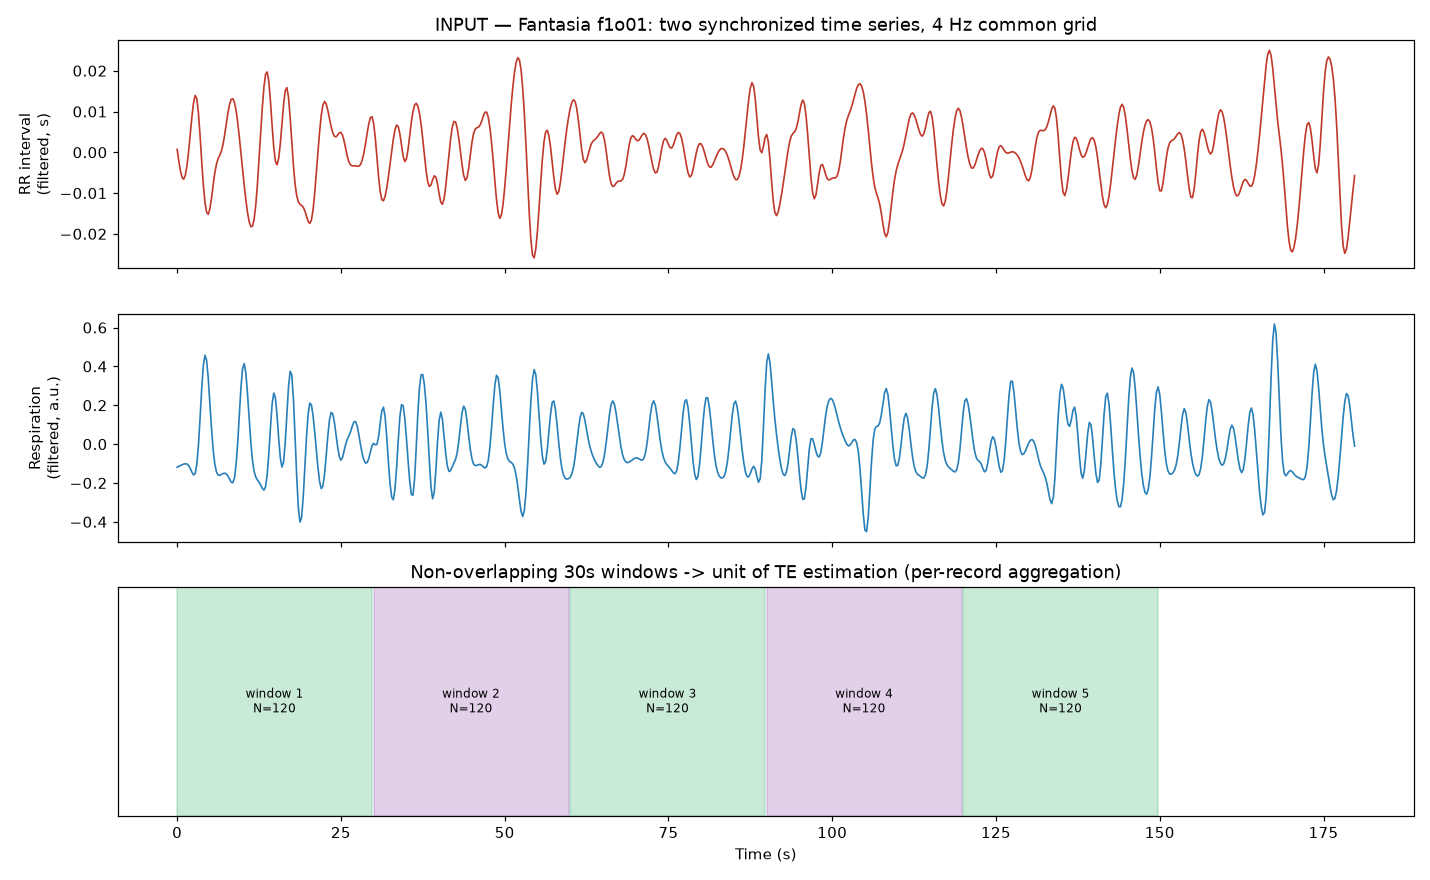
\includegraphics[width=\linewidth]{Fig/phase_t_input_output_signals.png}
    \caption{Representative time-series segments demonstrating the transition from synthetic linear and non-linear coupled systems to empirical Fantasia cardiorespiratory recordings, exhibiting prominent baseline wander and non-stationary dynamics.}
    \label{fig:dataset_signals}
\end{figure}

\subsection{Baseline Estimators for Comparison}
We compare our proposed amortized framework against established classical and modern deep learning methodologies:
\begin{itemize}
    \item \textbf{Linear VAR TE:} A parametric estimator assuming joint Gaussianity \cite{schreiber2000measuring}.
    \item \textbf{KSG Estimator ($k$-NN):} The non-parametric standard \cite{kraskov2004estimating} configured with $k=4$ neighbors, evaluated across all $N \in [10, 200]$.
    \item \textbf{Standard MINE (Disjoint MLPs):} An unconstrained ablation baseline employing two independent neural networks without weight sharing \cite{belghazi2018mine}.
    \item \textbf{TREET (Transformers, 2024/2025):} SOTA Transformer architecture using causal attention \cite{treet2024}.
    \item \textbf{TENDE (Score-based Diffusion SDE, 2026):} SOTA diffusion framework operating via VP-SDE score matching \cite{tende2025}.
\end{itemize}

\subsection{Training Configurations \& Adaptation Setup}
Pre-training on synthetic corpora utilized the Adam optimizer with learning rate $\eta = 10^{-3}$, batch size 256, and 100 epochs. For test-time Unsupervised Domain Adaptation on Fantasia windows, the shared statistics layers were adapted using stratified 5-fold cross-validation with learning rate $10^{-4}$ for 5 epochs. Quantum circuits were simulated in Python using PennyLane \cite{bergholm2018pennylane} via the \texttt{lightning.qubit} backend.
